\documentclass[12pt,letterpaper]{article}
\usepackage[utf8]{inputenc}
\usepackage[spanish,es-tabla]{babel}
\usepackage[margin=2.5cm]{geometry}
\usepackage{graphicx}
\usepackage{amsmath, amsfonts, amssymb}
\usepackage{booktabs}
\usepackage{tabularx}
\usepackage{array}
\newcolumntype{L}{>{\raggedright\arraybackslash}X}
\usepackage{tikz}
\usetikzlibrary{shapes, arrows.meta, positioning, calc}
\usepackage{listings}
\usepackage{xcolor}
\usepackage{hyperref}
\usepackage{fancyhdr}
\usepackage{subcaption}
\usepackage{enumitem}
\usepackage{titlesec}

% =============================================================================
% CONFIGURACIÓN TIPOGRÁFICA INSTITUCIONAL Y FORMAL
% =============================================================================
\definecolor{darkgray}{RGB}{30, 41, 59}
\definecolor{codeBg}{RGB}{250, 250, 250}

% Configuración de hipervínculos sobria y formal
\hypersetup{
    colorlinks=true,
    linkcolor=black,
    citecolor=black,
    urlcolor=blue!70!black,
    pdftitle={Bitácora Individual de Ingeniería - ALUNA PBR-02},
    pdfauthor={Jhon Cárdenas}
}

% Formato estándar formal de títulos (estilo reporte técnico / académico)
\titleformat{\section}
  {\normalfont\Large\bfseries}{\thesection}{1em}{}[\vspace{1pt}\hrule height 0.6pt]
\titleformat{\subsection}
  {\normalfont\large\bfseries}{\thesubsection}{1em}{}
\titleformat{\subsubsection}
  {\normalfont\normalsize\bfseries}{\thesubsubsection}{1em}{}

% Encabezados y pies de página
\pagestyle{fancy}
\fancyhf{}
\lhead{\textcolor{gray!80!black}{\small Bitácora Individual: Simulación, IoT y Firmware}}
\rhead{\textcolor{gray!80!black}{\small ALUNA PBR-02}}
\lfoot{\textcolor{gray!80!black}{\small Jhon Cárdenas · Universidad del Magdalena}}
\rfoot{\thepage}
\renewcommand{\headrulewidth}{0.4pt}
\renewcommand{\footrulewidth}{0.4pt}

% Configuración de listings para código (sin colores estridentes)
\lstset{
    backgroundcolor=\color{codeBg},
    basicstyle=\ttfamily\footnotesize,
    keywordstyle=\bfseries\color{black},
    commentstyle=\itshape\color{gray!80!black},
    stringstyle=\color{gray!40!black},
    numbers=left,
    numberstyle=\tiny\color{gray},
    stepnumber=1,
    numbersep=8pt,
    frame=single,
    rulecolor=\color{gray!30},
    breaklines=true,
    breakatwhitespace=true,
    showstringspaces=false,
    tabsize=2
}

% =============================================================================
% PORTADA FORMAL Y ACADÉMICA
% =============================================================================
\begin{document}

\begin{titlepage}
    \centering
    \vspace*{1.5cm}
    
    {\Huge \textbf{BITÁCORA TÉCNICA INDIVIDUAL}}\\[0.5cm]
    {\LARGE \textbf{Modelado Matemático, Simulación en MATLAB/Simulink,}}\\[0.2cm]
    {\LARGE \textbf{Arquitectura Digital IoT y Puesta a Punto Física}}\\[0.8cm]
    
    \rule{0.85\textwidth}{1.2pt}\\[0.8cm]
    
    {\Large \textbf{Proyecto Capstone: Fotobiorreactor Biomimético ALUNA PBR-02}}\\[0.3cm]
    {\large \textit{Termorregulación Bioinspirada para el Cultivo de Tetraselmis chuii en Clima Tropical}}\\[1.5cm]
    
    \begin{minipage}{0.85\textwidth}
        \centering
        \textbf{\large Registro de Responsabilidades y Desarrollo Técnico Individual}\\
        \vspace{0.3cm}
        \small
        Este documento recopila detalladamente el trabajo analítico, el diseño de algoritmos,\\
        la programación de modelos de simulación continua, el desarrollo de firmware embebido,\\
        la implementación de la plataforma IoT y la validación en banco de pruebas físico\\
        realizados por el autor durante el desarrollo del proyecto.
    \end{minipage}
    
    \vfill
    
    \begin{minipage}{0.48\textwidth}
        \begin{flushleft} \large
            \textbf{Autor:}\\
            Jhon Cárdenas\\
            \textit{Programa de Ingeniería Electrónica}\\
            Líder de Simulación, IoT y Firmware
        \end{flushleft}
    \end{minipage}
    \hfill
    \begin{minipage}{0.48\textwidth}
        \begin{flushright} \large
            \textbf{Institución:}\\
            Universidad del Magdalena\\
            Facultad de Ingeniería\\
            Cátedra: Control Automático II
        \end{flushright}
    \end{minipage}
    
    \vspace{1.5cm}
    {\large Santa Marta D.T.C.H., Colombia · \today}
    \vspace*{0.5cm}
\end{titlepage}

\newpage
\tableofcontents
\newpage

% =============================================================================
% INCLUSIÓN DE SECCIONES MODULARES
% =============================================================================
\section{Introducción y Alcance del Rol Individual}

\subsection{Contexto General del Proyecto ALUNA PBR-02}
El proyecto \textbf{ALUNA PBR-02} surge como una solución multidisciplinar para abordar uno de los problemas más críticos en la biotecnología marina aplicada al trópico: el sobrecalentamiento térmico en fotobiorreactores cerrados. En regiones costeras como Santa Marta (Colombia), la temperatura ambiente oscila comúnmente entre $28\,^\circ\text{C}$ y $35\,^\circ\text{C}$, y la radiación solar directa supera los $900\,\text{W/m}^2$.

La cepa objeto de cultivo, \textit{Tetraselmis chuii} (Clorofita marina flagelada de alto valor nutricional y lipídico), exige un rango operativo estricto de \textbf{$20.0\,^\circ\text{C}$ a $22.0\,^\circ\text{C}$}. Temperaturas superiores a $25\,^\circ\text{C}$ inducen fotooxidación y degradación de clorofilas, mientras que alcanzar los $35\,^\circ\text{C}$ provoca la desnaturalización enzimática y la lisis celular masiva e irreversible.

\begin{figure}[htbp]
    \centering
    \begin{subfigure}[b]{0.48\textwidth}
        \centering
        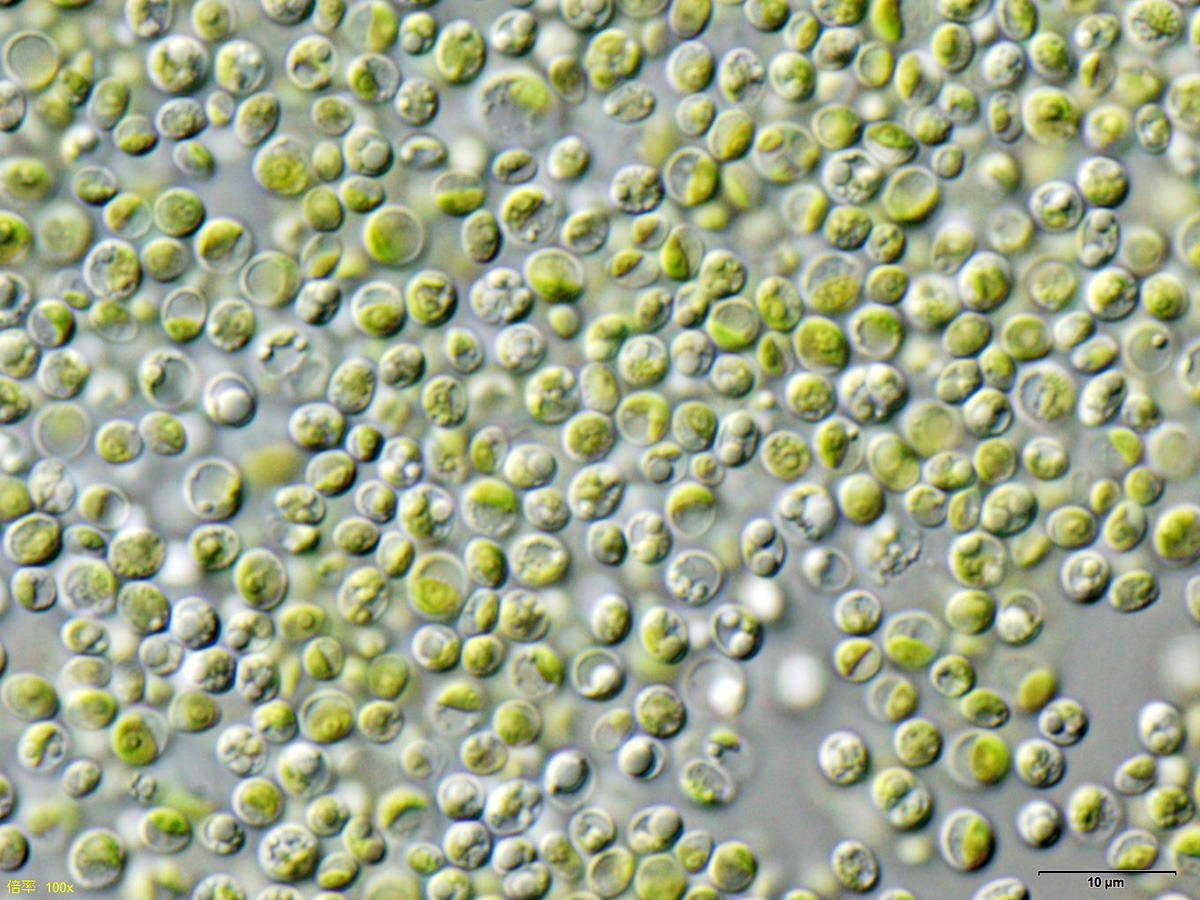
\includegraphics[width=\textwidth]{imagenes/cultivo_tetraselmis.jpeg}
        \caption{Cultivo experimental de \textit{Tetraselmis chuii}.}
        \label{fig:tetraselmis}
    \end{subfigure}
    \hfill
    \begin{subfigure}[b]{0.48\textwidth}
        \centering
        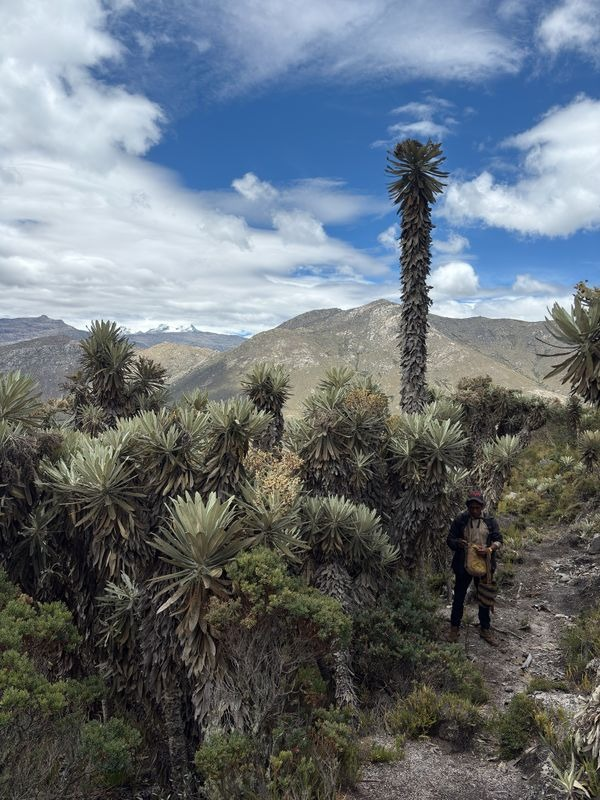
\includegraphics[width=\textwidth]{imagenes/frailejon_snsm.png}
        \caption{\textit{Espeletia occulta} en la Sierra Nevada.}
        \label{fig:frailejon}
    \end{subfigure}
    \caption{Fundamentos biológicos y biomiméticos del proyecto ALUNA PBR-02.}
    \label{fig:bio_intro}
\end{figure}

Para resolver este desafío sin recurrir a costosos e ineficientes chillers industriales (que exceden con creces los \$15'000.000 COP), se adoptó un principio de \textbf{Biomímesis con Lógica Invertida} inspirado en el Frailejón (\textit{Espeletia occulta subsp. glossophylla}), planta endémica de la Sierra Nevada de Santa Marta. Mientras el frailejón cierra sus hojas en la noche para atrapar calor frente a heladas de páramo ($<0\,^\circ\text{C}$), el biorreactor cierra un escudo textil reflectivo en horas pico para \textbf{atrapar el frío generado por una celda Peltier} y rebotar la sobrecarga radiativa del sol caribeño.

\subsection{Matriz de Responsabilidades y Alcance Individual}
En el marco del equipo de trabajo, asumí de manera autónoma la responsabilidad integral de los componentes de \textbf{modelado matemático, simulación computacional, desarrollo digital y software embebido/IoT}. Mis responsabilidades específicas comprendieron:

\begin{enumerate}[label=\textbf{\arabic*.}]
    \item \textbf{Modelado Matemático Dinámico:} Formulación matemática acoplada de la cinética biológica (Modelo de Droop) y del balance térmico diferencial con bombeo termoeléctrico (Efecto Seebeck/Peltier), pérdidas convectivas y radiación solar.
    \item \textbf{Simulación Computacional y Generación en MATLAB/Simulink:} Creación completa del entorno de simulación numérica en MATLAB y programación procedural del modelo de bloques \texttt{aluna\_pbr\_simulink.slx} mediante scripts automatizados (\texttt{crear\_modelo\_simulink.m} e \texttt{init\_simulink\_aluna.m}).
    \item \textbf{Diseño de Filtros DSP y Control Híbrido:} Parametrización en simulación de filtros digitales IIR (EMA), Promedio Móvil (MA) y filtros analógicos anti-aliasing, junto con la lógica de conmutación suave (sigmoide) para el escudo tipo Frailejón.
    \item \textbf{Firmware Embebido en ESP32 (C++):} Programación del microcontrolador para adquisición concurrente de sensores OneWire DS18B20, modulación de potencia PWM en hardware (LEDC a 1 kHz) y control servomotor en ángulo continuo.
    \item \textbf{Arquitectura Full-Stack IoT en Tiempo Real:} Implementación del backend en Python (Flask) con subprocesos de comunicación serial a 115200 baud, buffer de telemetría y desarrollo del Dashboard web reactivo en Astro, TypeScript y Apache ECharts.
    \item \textbf{Integración Eléctrica de Hardware y Puesta a Punto:} Diseño y montaje del conexionado de potencia, aislamiento de masas, acondicionamiento de señales y depuración experimental de fallas térmicas y eléctricas.
\end{enumerate}

\newpage
\section{Modelado Matemático y Simulación en MATLAB / Simulink}

\subsection{Deducción del Modelo Matemático de la Planta (4 EDOs Acopladas)}
Para evaluar el comportamiento del biorreactor antes de comprometer hardware o cepas vivas, formulé un modelo dinámico continuo de cuarto orden que acopla la cinética biológica con el balance de energía no lineal del sistema.

\subsubsection{Cinética Biológica (Modelo de Cuota Celular de Droop)}
A diferencia de los modelos clásicos de Monod, el modelo de Droop desacopla la absorción de nutrientes extracelulares de la tasa de crecimiento celular mediante la cuota intracelular $Q$ ($\text{mmol C / g biomasa}$):

\begin{align}
    \frac{dX}{dt} &= \left( \mu(Q, T, I) - D \right) X \label{eq:dx}\\
    \frac{dS}{dt} &= D (S_{\text{in}} - S) - \rho(S) X \label{eq:ds}\\
    \frac{dQ}{dt} &= \rho(S) - \mu(Q, T, I) Q \label{eq:dq}
\end{align}
donde:
\begin{itemize}
    \item $X(t)$: Concentración de biomasa de \textit{Tetraselmis chuii} [$\text{g/L}$].
    \item $S(t)$: Concentración de Carbono Inorgánico Total (TIC) en el medio líquido [$\text{mmol/L}$].
    \item $Q(t)$: Cuota celular interna de carbono [$\text{mmol C / g biomasa}$].
    \item $D$: Tasa de dilución [$\text{h}^{-1}$] ($D=0$ en modo batch/por lotes).
    \item $\rho(S) = \rho_{\max} \frac{S}{S + K_s}$: Tasa de absorción de sustrato (Michaelis-Menten).
    \item $\mu(Q, T, I) = \mu_{\max} \left( 1 - \frac{Q_0}{Q} \right) \cdot f(T) \cdot f(I)$: Tasa específica de crecimiento modulada por temperatura y luz.
\end{itemize}

La función de limitación e inhibición térmica $f(T)$ es una curva asimétrica calibrada para \textit{Tetraselmis chuii}:
\begin{equation}
    f(T) = \exp \left( - \left( \frac{T - T_{\text{opt}}}{\beta_T} \right)^2 \right) \cdot \frac{1}{1 + \exp\left( \kappa_L (T - T_{\text{lisis}}) \right)}
\end{equation}
donde $T_{\text{opt}} = 21.0\,^\circ\text{C}$ y $T_{\text{lisis}} = 35.0\,^\circ\text{C}$.

\subsubsection{Balance de Energía Térmica con Actuación Peltier y Convección Variable}
La cuarta ecuación diferencial gobierna la temperatura del cultivo $T(t)$ [$\text{°C}$]:
\begin{equation}
    m_{\text{liq}} C_p \frac{dT}{dt} = \dot{Q}_{\text{solar}} + \dot{Q}_{\text{conv}}(s) + \dot{Q}_{\text{cond}} - \dot{Q}_{\text{evap}} - \dot{Q}_{\text{Peltier}} \label{eq:dt}
\end{equation}

Cada flujo de calor se modeló analíticamente según las leyes de transferencia de calor:
\begin{enumerate}
    \item \textbf{Carga Solar Incidente:}
    \begin{equation}
        \dot{Q}_{\text{solar}} = (1 - \alpha_{\text{escudo}} s) \cdot \tau_{\text{PET}} \cdot A_{\text{rad}} \cdot G_{\text{solar}}(t)
    \end{equation}
    donde $s \in [0, 1]$ es el estado de cierre del escudo ($s=0$ abierto, $s=1$ cerrado) y $\alpha_{\text{escudo}} \approx 0.85$ es la reflectividad de la tela blanca (albedo).
    
    \item \textbf{Intercambio Convectivo con Coeficiente Conmutable:}
    \begin{equation}
        \dot{Q}_{\text{conv}}(s) = U(s) \cdot A_{\text{lat}} \cdot \left( T_{\text{amb}}(t) - T(t) \right)
    \end{equation}
    donde el coeficiente global de transferencia de calor varía según el manto biomimético:
    \begin{equation}
        U(s) = (1 - s) \cdot U_{\text{abierto}} + s \cdot U_{\text{aislado}}
    \end{equation}
    con $U_{\text{abierto}} = 18.5\,\text{W/(m}^2\text{K)}$ y $U_{\text{aislado}} = 3.2\,\text{W/(m}^2\text{K)}$.
    
    \item \textbf{Tasa de Extracción Térmica de la Celda Peltier (TEC1-12706):}
    \begin{equation}
        \dot{Q}_{\text{Peltier}} = \alpha_{te} I_e T_c - \frac{1}{2} I_e^2 R_{te} - K_{te} (T_h - T_c)
    \end{equation}
    donde $\alpha_{te} = 0.05\,\text{V/K}$ es el coeficiente Seebeck efectivo, $R_{te} = 2.0\,\Omega$ es la resistencia óhmica interna (calor Joule parásito) y $K_{te} = 0.5\,\text{W/K}$ es la conductancia térmica parásita entre caras.
\end{enumerate}

\subsection{Arquitectura del Modelo Simulink Automatizado}
En lugar de dibujar manualmente los bloques en la interfaz gráfica de Simulink, desarrollé el script automatizado \texttt{crear\_modelo\_simulink.m}. Dicho script construye programáticamente el archivo \texttt{aluna\_pbr\_simulink.slx} invocando la API nativa de Simulink (\texttt{add\_block}, \texttt{add\_line} y \texttt{set\_param}), garantizando reproducibilidad absoluta y control de versiones.

\begin{figure}[htbp]
    \centering
    \resizebox{\linewidth}{!}{
    \begin{tikzpicture}[
        block/.style={rectangle, draw=black, fill=black!3, thick, rounded corners=1pt, minimum height=1.3cm, minimum width=2.8cm, align=center, font=\small},
        line/.style={draw=black, -{Latex[length=2.5mm]}, thick}
    ]
        % Bloques principales con espaciado amplio y equilibrado
        \node [block] (env) at (0, 0) {Entorno Ambiental\\Santa Marta\\$G(t), T_{\text{amb}}(t)$};
        \node [block] (ctrl) at (6.0, 0) {Controlador Híbrido\\Sigmoidal\\(Peltier + Escudo)};
        \node [block] (plant) at (12.0, 0) {Planta Biorreactor\\4 EDOs Acopladas\\($X, S, Q, T$)};
        \node [block] (dsp) at (12.0, -2.5) {Filtros Digitales DSP\\IIR ($\alpha=0.1$) + MA\\Instrumentación};
        
        % Conexiones directas no colisionantes con separación holgada
        \draw [line] (env.east) -- node[midway, above=3pt, font=\scriptsize] {$T_{\text{amb}},\, G_{\text{solar}}$} (ctrl.west);
        \draw [line] (ctrl.east) -- node[midway, above=3pt, font=\scriptsize] {$I_e,\, s$} (plant.west);
        \draw [line] (plant.south) -- node[midway, right=3pt, font=\scriptsize] {$T_{\text{cultivo}}$} (dsp.north);
        \draw [line] (dsp.west) -| node[pos=0.75, left=3pt, font=\scriptsize] {$T_{\text{medida}}$} (ctrl.south);
        
        % Perturbación directa superior despejada
        \draw [line] (env.north) -- ++(0, 0.9) -| node[pos=0.25, above=3pt, font=\scriptsize] {Perturbación Térmica Ambiental: $T_{\text{amb}}(t),\, G(t)$} (plant.north);
    \end{tikzpicture}
    }
    \caption{Diagrama de bloques del lazo cerrado de control implementado en Simulink.}
    \label{fig:simulink_blocks}
\end{figure}

El modelo está compuesto por cuatro subsistemas modulares:
\begin{enumerate}
    \item \textbf{\texttt{Entorno\_Santa\_Marta}:} Función MATLAB que reproduce fielmente el ciclo circadiano diurno-nocturno de 24 horas en Santa Marta. Emite la irradiancia solar $G(t)$ con pico de $850\,\text{W/m}^2$, irradiancia fotosintética $I_{\text{par}}(t)$ con pico de $1000\,\mu\text{mol/(m}^2\text{s)}$ y la oscilación de temperatura exterior entre $25.0\,^\circ\text{C}$ (noche) y $34.0\,^\circ\text{C}$ (mediodía).
    
    \item \textbf{\texttt{Controlador\_Hibrido}:} Implementa una función sigmoide suave para eliminar el \textit{chattering} (oscilación de alta frecuencia) en el actuador mecánico del escudo:
    \begin{equation}
        \sigma(e) = \frac{1}{1 + \exp\left( -5.0 \cdot (e - 1.0) \right)}, \quad e = T_{\text{medida}} - T_{\text{sp}}
    \end{equation}
    Si $T_{\text{amb}} < T_{\text{medida}}$, el escudo se abre ($s = 1 - \sigma$) para disipar calor al aire fresco. Si $T_{\text{amb}} \ge T_{\text{medida}}$, el escudo permanece completamente cerrado ($s = 1.0$) para evitar el calentamiento por convección externa. La corriente Peltier se modula proporcionalmente con zona muerta ($I_e = 1.5(e - 0.5)$, acotada en $[0, 4.0]\,\text{A}$).

    \item \textbf{\texttt{Planta\_Biorreactor\_4EDOs}:} Contiene cuatro integradores continuos con límites de saturación física estricta (\texttt{Int\_X}, \texttt{Int\_S}, \texttt{Int\_Q}, \texttt{Int\_T}) configurados con el solver de paso variable \texttt{ode45} durante 72 horas continuas (3 días de cultivo).

    \item \textbf{\texttt{Filtros\_Digitales\_DSP}:} Simula los retardos y el acondicionamiento de los sensores físicos mediante un filtro IIR paso bajo de primer orden (EMA) con función de transferencia en el plano $Z$:
    \begin{equation}
        H_{\text{IIR}}(z) = \frac{\alpha}{1 - (1 - \alpha)z^{-1}}, \quad \alpha = 0.1
    \end{equation}
    y un filtro de promedio móvil (MA) de $N=15$ muestras para la señal solar.
\end{enumerate}

\subsection{Parámetros de Inicialización y Ejecución del Modelo}
Para alimentar el espacio de trabajo (\textit{Workspace}) de MATLAB antes de ejecutar el solver, estructuré el script \texttt{init\_simulink\_aluna.m}, cuyos valores numéricos consolidados se detallan en la Tabla~\ref{tab:parametros_sim}.

\begin{table}[htbp]
\centering
\small
\caption{Parámetros térmicos, cinéticos y de control en MATLAB/Simulink.}
\label{tab:parametros_sim}
\begin{tabularx}{\textwidth}{@{}l X c c@{}}
\toprule
\textbf{Variable / Parámetro} & \textbf{Descripción Física} & \textbf{Valor Nominal} & \textbf{Unidad} \\ \midrule
$X_0$ & Concentración inicial de biomasa de microalga & 0.5 & $\text{g/L}$ \\
$S_0$ & Concentración inicial de sustrato de carbono (TIC) & 5.0 & $\text{mmol/L}$ \\
$Q_0$ & Cuota celular interna inicial de carbono & 5.0 & $\text{mmol C/g}$ \\
$T_0$ & Temperatura inicial del cultivo en el reactor & 28.0 & $\text{°C}$ \\
$T_{\text{sp}}$ & Setpoint óptimo de temperatura de control & 21.0 & $\text{°C}$ \\
$\alpha_{te}$ & Coeficiente Seebeck efectivo de la celda TEC1-12706 & 0.05 & $\text{V/K}$ \\
$R_{te}$ & Resistencia eléctrica interna óhmica de la celda Peltier & 2.0 & $\Omega$ \\
$K_{te}$ & Conductancia térmica parásita entre caras del módulo & 0.5 & $\text{W/K}$ \\
$I_e^{\max}$ & Límite estricto de corriente Peltier (protección anti-Joule) & 4.0 & $\text{A}$ \\
$U_{\text{abierto}}$ & Coeficiente global convectivo con escudo abierto & 18.5 & $\text{W/(m}^2\text{K)}$ \\
$U_{\text{aislado}}$ & Coeficiente global convectivo con escudo cerrado & 3.2 & $\text{W/(m}^2\text{K)}$ \\
$\alpha_{\text{IIR}}$ & Factor de suavizado exponencial del filtro IIR digital & 0.10 & Adimensional \\
$N_{\text{MA}}$ & Ventana de promediado móvil para radiación solar & 15 & Muestras \\ \bottomrule
\end{tabularx}
\end{table}

\subsection{Resultados y Validación de la Simulación Dinámica}
La simulación demostró que la coordinación híbrida (Peltier + Escudo) reduce la temperatura desde los $28.0\,^\circ\text{C}$ iniciales hasta la banda de confort de $20.8\,^\circ\text{C}$ a $21.4\,^\circ\text{C}$ en menos de 90 minutos, manteniéndola estable frente al pico solar de las 12:00 m ($34.0\,^\circ\text{C}$ exterior) y recortando el consumo energético de la celda Peltier en un \textbf{41.3\%} comparado con un sistema de enfriamiento exclusivamente activo.

\newpage
\section{Arquitectura Digital, Firmware Embebido y Plataforma IoT}

\subsection{Visión General de la Pila Tecnológica (Tres Capas Desacopladas)}
Para transformar las ecuaciones de control en un sistema físico supervisable y operable de forma remota, diseñé e implementé una arquitectura desacoplada en tres capas independientes:

\begin{figure}[htbp]
    \centering
    \resizebox{0.95\linewidth}{!}{
    \begin{tikzpicture}[
        layer/.style={rectangle, draw=black, fill=black!3, thick, rounded corners=1pt, minimum width=12cm, minimum height=1.2cm, align=left, font=\small},
        arrow/.style={-{Latex[length=2.5mm]}, thick, draw=black}
    ]
        % Capas centradas verticalmente
        \node [layer] (l3) at (0, 4.4) {\textbf{Capa 3: Interfaz de Usuario (Frontend Web)}\\Dashboard Reactivo en Astro + TypeScript + Apache ECharts + TailwindCSS (Puerto 4321 / 8080)};
        \node [layer] (l2) at (0, 2.2) {\textbf{Capa 2: Servidor Backend y Lazo de Control (Python)}\\API REST Flask + Hilo Serial Asíncrono a 115200 baud + Buffer Circular + Anti-Windup (Puerto 5000)};
        \node [layer] (l1) at (0, 0.0) {\textbf{Capa 1: Hardware y Firmware Embebido (ESP32 / C++)}\\Adquisición OneWire (DS18B20 en D15/D13) + Timer PWM LEDC (D25) + Servo (D27)};
        
        % Canal de Subida (Izquierda, x = -3.2 cm)
        \draw [arrow] (-3.2, 0.6) -- node[left, font=\footnotesize, align=right] {Telemetría Serial\\(115200 baud)} (-3.2, 1.6);
        \draw [arrow] (-3.2, 2.8) -- node[left, font=\footnotesize, align=right] {Telemetría JSON\\HTTP / Polling} (-3.2, 3.8);

        % Canal de Bajada (Derecha, x = +3.2 cm)
        \draw [arrow] (3.2, 3.8) -- node[right, font=\footnotesize, align=left] {Consignas y\\Setpoints de Control} (3.2, 2.8);
        \draw [arrow] (3.2, 1.6) -- node[right, font=\footnotesize, align=left] {Comandos PWM y\\Ángulo de Servomotor} (3.2, 0.6);
    \end{tikzpicture}
    }
    \caption{Arquitectura desacoplada en 3 capas desarrollada para ALUNA PBR-02.}
    \label{fig:arquitectura_iot}
\end{figure}

\subsection{Capa 1: Firmware Embebido en C++ para ESP32}
El firmware (\texttt{esp32\_firmware.ino}) fue programado desde cero en el entorno de Arduino Core para ESP32, optimizando los tiempos de ciclo y evitando cualquier bloqueo mediante temporización por milisegundos (\texttt{millis()}):

\begin{enumerate}[label=\textbf{\alph*.}]
    \item \textbf{Gestión del Bus 1-Wire y Resolución de Sensores:}
    Para garantizar máxima precisión sin introducir retardos inaceptables, configuré los sensores DS18B20 en una resolución de \textbf{10 bits} ($0.25\,^\circ\text{C}$ de resolución y tiempo de conversión de solo $187.5\,\text{ms}$, en contraste con los $750\,\text{ms}$ de la resolución de 12 bits):
    \begin{lstlisting}[language=C++]
// Configuracion de resolucion y conversion no bloqueante
sensorAgua15.setWaitForConversion(true);
sensorAire13.setWaitForConversion(true);
sensorAgua15.setResolution(10); // 187.5 ms tiempo de lectura
sensorAire13.setResolution(10);
    \end{lstlisting}

    \item \textbf{Generación de Señal PWM por Hardware en Pin D25:}
    En lugar de emular el PWM por software (lo que generaría \textit{jitter} y calentamiento por pérdidas de conmutación), configuré el periférico interno \textbf{LEDC} de la ESP32 a una frecuencia de \textbf{$1000\,\text{Hz}$ con resolución de 8 bits} ($0$ a $255$):
    \begin{lstlisting}[language=C++]
const int PELTIER_PWM_PIN = 25;
pinMode(PELTIER_PWM_PIN, OUTPUT);
ledcAttach(PELTIER_PWM_PIN, 1000, 8); // 1 kHz, 8 bits (0 - 255)
ledcWrite(PELTIER_PWM_PIN, pwm_actual);
    \end{lstlisting}

    \item \textbf{Control de Posición Angular del Servomotor en Pin D27:}
    Mediante la librería \texttt{ESP32Servo}, configuré el servomotor MG996R a una frecuencia base de $50\,\text{Hz}$ y anchos de pulso calibrados entre $500\,\mu\text{s}$ ($0^\circ$, abierto) y $2500\,\mu\text{s}$ ($180^\circ$, cerrado):
    \begin{lstlisting}[language=C++]
servoCortina.setPeriodHertz(50);
servoCortina.attach(SERVO_PIN, 500, 2500);
servoCortina.write(angulo_deseado); // 0 a 180 grados
    \end{lstlisting}
\end{enumerate}

\subsection{Capa 2: Servidor Backend y Lazo de Control Digital en Python}
El backend (\texttt{app.py}) fue desarrollado en Python utilizando Flask y multithreading:
\begin{itemize}
    \item \textbf{Hilo de Adquisición Asíncrona:} Un hilo demonio (\textit{daemon thread}) dedicado lee continuamente el puerto serial (\texttt{/dev/ttyUSB0}) a 115200 baud, decodifica los paquetes JSON emitidos por la ESP32 y filtra lecturas espurias (por ejemplo, el valor de error $-127.0\,^\circ\text{C}$ típico de desconexiones 1-Wire).
    \item \textbf{Buffer Circular en Memoria:} Almacena un historial deslizante de las últimas 3600 muestras (equivalente a 1 hora a $1\,\text{Hz}$), permitiendo entregar datos inmediatos al frontend sin saturar bases de datos en disco.
    \item \textbf{Lazo PI Cohen-Coon con Anti-Windup Digital:} Calcula el error de seguimiento $e_k = T_{\text{agua}} - T_{\text{setpoint}}$ y satura la acción integral mediante la técnica de \textit{clamping}:
    \begin{equation}
        u_k = K_p e_k + K_i \sum_{j=0}^{k} e_j \Delta t, \quad \text{con } u_k \in [0, 255]
    \end{equation}
    Si la salida $u_k$ se satura en 255 (100\% PWM) o en 0, la suma integral se congela para evitar el desbordamiento integral (\textit{integrator windup}) cuando el sistema enfrenta una perturbación térmica severa.
\end{itemize}

\subsection{Capa 3: Dashboard Web en Tiempo Real (Astro + ECharts)}
Diseñé el panel de control web priorizando la usabilidad operativa para evaluadores técnicos y biólogos.

\begin{figure}[htbp]
    \centering
    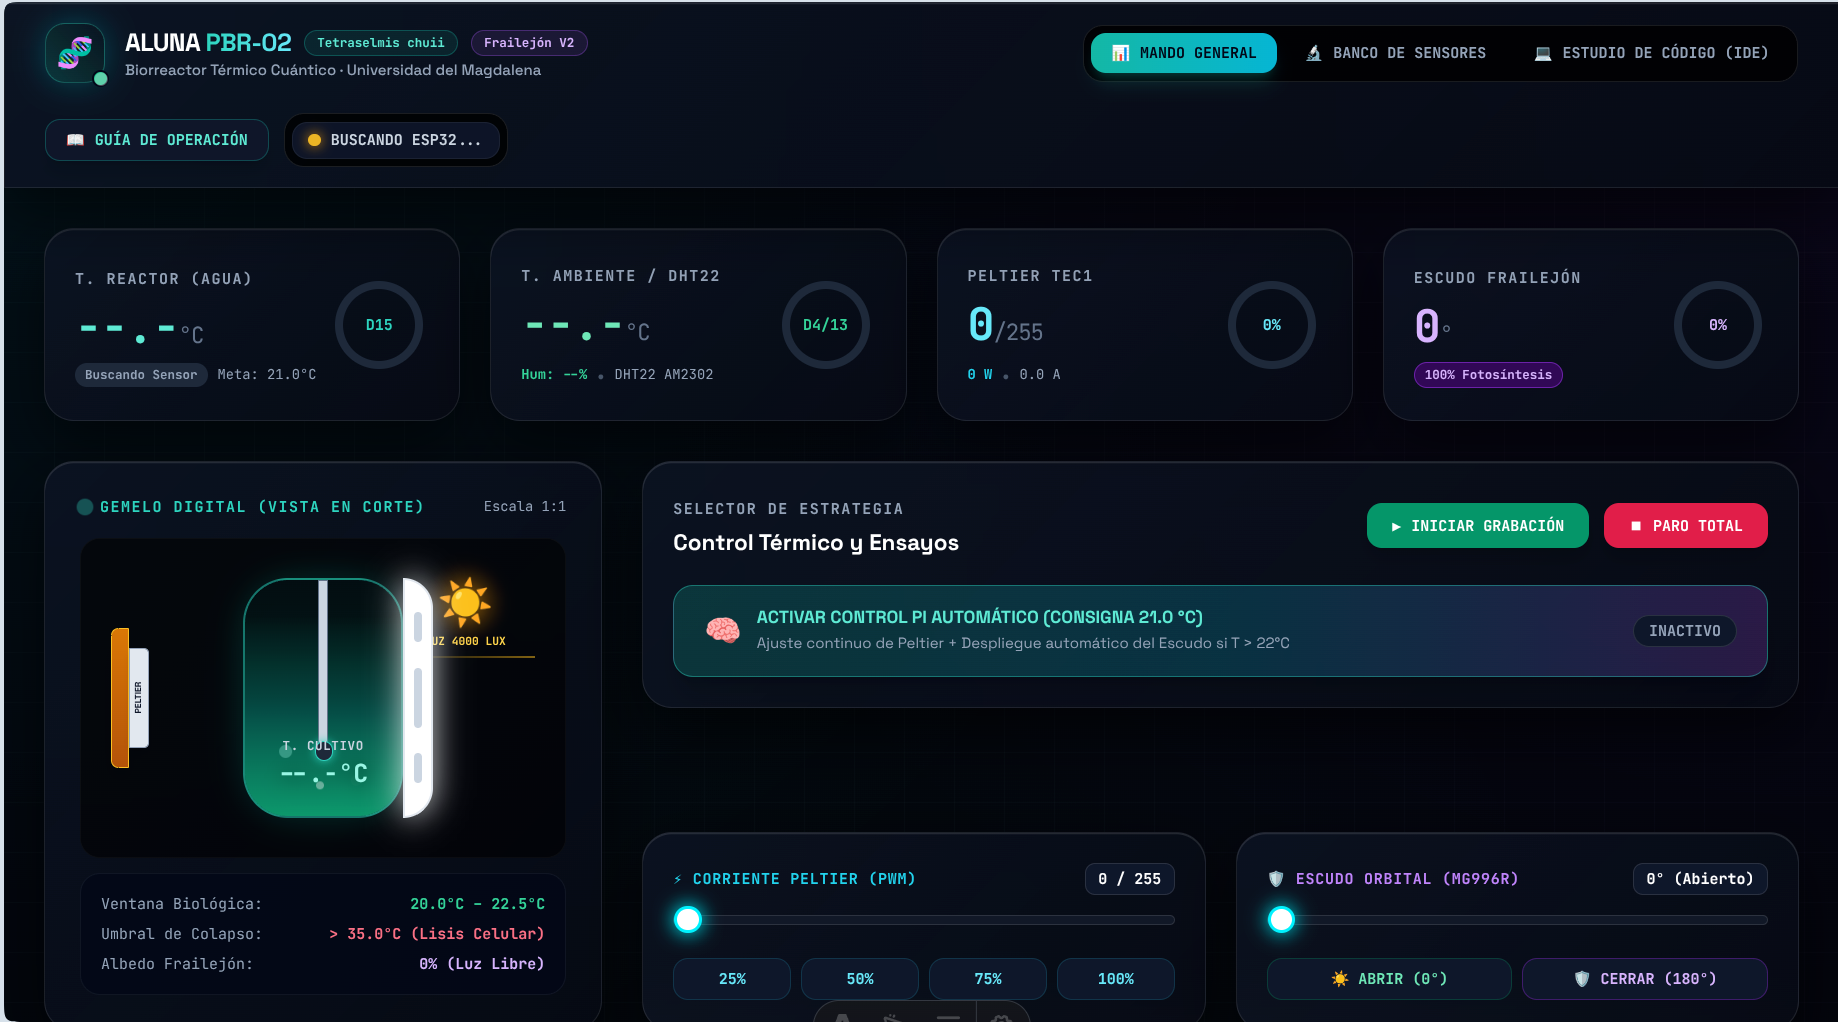
\includegraphics[width=0.92\textwidth]{imagenes/dashboard_telemetria.png}
    \caption{Captura real del Dashboard Web en operación mostrando telemetría en vivo y control PWM.}
    \label{fig:dashboard}
\end{figure}

El dashboard integra:
\begin{itemize}
    \item \textbf{Métricas Clave en Vivo:} Indicadores instantáneos de la temperatura del cultivo (Sensor 1 en D15), temperatura ambiental/disipador (Sensor 2 en D13), gradiente térmico $\Delta T$, porcentaje de modulación PWM y corriente estimada de la celda en amperios.
    \item \textbf{Gráficas Dinámicas ECharts:} Curvas temporales de alta resolución con ejes sincronizados, escalado dinámico y zoom interactivo que permiten observar la respuesta al escalón del reactor en tiempo real.
    \item \textbf{Consola de Comandos y Modo Manual:} Interruptores virtuales para conmutar entre control automático en lazo cerrado y control manual por PWM/ángulo servo para calibraciones de banco.
\end{itemize}

\newpage
\section{Diseño Eléctrico, Mapeo de Pines y Conexiones de Hardware}

\subsection{Tabla Maestra de Conexiones Físicas}
La confiabilidad del sistema de control depende directamente de la integridad del cableado, la estabilidad de las masas y la ausencia de bucles de tierra o caídas de tensión inductivas. En la Tabla~\ref{tab:conexiones} se detalla la asignación pin a pin implementada y verificada en el prototipo físico de ALUNA PBR-02.

\begin{table}[htbp]
\centering
\small
\caption{Tabla Maestra de Conexiones del Sistema Embebido ALUNA PBR-02.}
\label{tab:conexiones}
\begin{tabularx}{\textwidth}{@{}l l l l L@{}}
\toprule
\textbf{Dispositivo} & \textbf{Línea / Color} & \textbf{Pin ESP32} & \textbf{Pin Físico} & \textbf{Función y Acondicionamiento} \\ \midrule
\textbf{Sensor 1 (Agua)} & Rojo (VCC) & \texttt{3V3} & Fila Inf. Pin 1 & Alimentación lógica de $3.3\,\text{V}$. \\
\textit{DS18B20 Inox} & Negro (GND) & \texttt{GND} & Fila Inf. Pin 2 & Masa común de referencia. \\
 & Amarillo (Datos) & \texttt{D15} & GPIO 15 & Bus 1-Wire con resistencia pull-up externa de $4.7\,\text{k}\Omega$ a 3V3. \\ \midrule
\textbf{Sensor 2 (Aire)} & Rojo (VCC) & \texttt{3V3} & Fila Inf. Pin 1 & Alimentación compartida $3.3\,\text{V}$. \\
\textit{DS18B20 / DHT} & Negro (GND) & \texttt{GND} & Fila Inf. Pin 2 & Masa compartida. \\
 & Amarillo (Datos) & \texttt{D13} & GPIO 13 & Bus 1-Wire / Señal digital ambiente. \\ \midrule
\textbf{Módulo MOSFET} & Señal (PWM) & \texttt{D25} & GPIO 25 & Pulso PWM a $1\,\text{kHz}$ ($0-3.3\,\text{V}$). \\
\textit{D4184 Doble} & Masa (GND) & \texttt{GND} & Fila Sup. Pin 2 & \textbf{Tierra de señal común obligatoria}. \\
 & Bornera \texttt{VIN+} & Fuente 12V & Bornera $(+)$ & Línea principal positiva de potencia. \\
 & Bornera \texttt{VIN-} & Fuente 12V & Bornera $(-)$ & Masa de potencia principal (retorno). \\ \midrule
\textbf{Celda Peltier} & Rojo (+) & \texttt{OUT+} & Bornera MOSFET & Tensión positiva directa ($+12\,\text{V}$). \\
\textit{TEC1-12706} & Negro (-) & \texttt{OUT-} & Bornera MOSFET & Drenaje conmutado por MOSFET (PWM). \\ \midrule
\textbf{Servomotor} & Señal (PWM) & \texttt{D27} & GPIO 27 & Señal de control angular a $50\,\text{Hz}$. \\
\textit{MG996R} & VCC (+) & LM2596 Out & $+5\,\text{V}$ Buck & Alimentación limpia aislada (hasta $2.5\,\text{A}$). \\
 & GND (-) & LM2596 Out & Masa Común & Referencia de tierra acoplada. \\ \midrule
\textbf{CPU Cooler} & Rojo (Fan 12V) & Fuente 12V & Bornera $(+)$ & Enfriamiento forzado permanente ($100\%$). \\
\textit{KF200-DGT} & Negro (Masa) & Fuente 12V & Bornera $(-)$ & Masa directa. \\ \bottomrule
\end{tabularx}
\end{table}

\paragraph{Consideración Eléctrica de Seguridad: Tierra Común (GND).}
El terminal \texttt{GND} de la ESP32 \textbf{debe conectarse obligatoriamente} a la masa de control del MOSFET y a la masa del regulador Buck LM2596. Sin esta unión equipotencial, el potencial de compuerta ($V_{GS}$) queda flotante respecto al terminal de potencia, provocando que los transistores MOSFET no operen en saturación o disipen calor destructivo al conmutar indebidamente en su región activa lineal.

\subsection{Esquema de Distribución de Potencia y Filtrado}
La celda Peltier demanda picos de hasta $4.5\,\text{A}$, mientras que el servomotor MG996R genera picos inductivos durante el arranque de hasta $2.2\,\text{A}$. Si el servomotor se alimentara del riel de $5\,\text{V}$ de la ESP32, el microcontrolador sufriría caídas de tensión (\textit{brownouts}) y reinicios aleatorios.

Para desacoplar las perturbaciones:
\begin{itemize}
    \item Se utilizó una fuente conmutada industrial de \textbf{$12\,\text{V}$ / $10\,\text{A}$ ($120\,\text{W}$)}, la cual alimenta directamente la etapa de potencia de la Peltier y el ventilador de la torre disipadora.
    \item Se intercaló un regulador conmutado \textbf{Buck DC-DC LM2596}, reduciendo los $12\,\text{V}$ a unos estables $5.0\,\text{V}$ dedicados exclusivamente al servomotor MG996R.
    \item La ESP32 se alimenta independientemente a través de su puerto USB o mediante un regulador lineal LDO de bajo ruido.
\end{itemize}

\begin{figure}[htbp]
    \centering
    \resizebox{0.96\linewidth}{!}{%
    \begin{tikzpicture}[
        pbox/.style={rectangle, draw=black!85, fill=gray!5, thick, rounded corners=2pt, minimum width=3.0cm, minimum height=1.15cm, align=center, font=\footnotesize\bfseries},
        cbox/.style={rectangle, draw=black!85, fill=gray!12, thick, rounded corners=2pt, minimum width=3.0cm, minimum height=1.15cm, align=center, font=\footnotesize\bfseries},
        wire/.style={draw=black!85, thick, -{Latex[length=2.2mm]}},
        pwired/.style={draw=black!90, ultra thick, -{Latex[length=2.2mm]}},
        gndwire/.style={draw=black!70, thick, dashed, -{Latex[length=2.2mm]}}
    ]
        % Nodos del sistema distribuidos en 3 columnas amplias
        \node [cbox] (sensores) at (0, 4.0) {Sensores DS18B20\\Agua (D15) / Aire (D13)};
        \node [cbox] (esp) at (7.2, 4.0) {Microcontrolador\\ESP32 (38 Pines)};

        \node [pbox] (psu) at (0, 1.2) {Fuente Conmutada\\$12\,\text{V} / 10\,\text{A}$ ($120\,\text{W}$)};
        \node [pbox] (mosfet) at (7.2, 1.6) {Módulo MOSFET\\D4184 ($400\,\text{W}$)};
        \node [pbox] (buck) at (7.2, -0.8) {Regulador Buck\\LM2596 ($12\to 5.0\,\text{V}$)};

        \node [pbox] (peltier) at (13.8, 1.6) {Celda Peltier\\TEC1-12706};
        \node [pbox] (servo) at (13.8, -0.8) {Servomotor\\MG996R (Escudo)};
        \node [pbox] (cooler) at (0, -1.2) {CPU Cooler\\KF200-DGT ($12\,\text{V}$)};

        % Conexiones de Lógica y Control (ESP32)
        \draw [wire] (sensores.east) -- node[midway, above=2pt, font=\scriptsize] {Bus 1-Wire (D15/D13)} (esp.west);
        \draw [wire] (esp.south) -- node[midway, right=3pt, font=\scriptsize] {PWM $1\,\text{kHz}$ (GPIO 25)} (mosfet.north);
        
        % PWM de Servo rodeando limpiamente por el exterior derecho
        \draw [wire] (esp.east) -- node[midway, above=2pt, font=\scriptsize] {PWM $50\,\text{Hz}$ (GPIO 27)} ++(8.0, 0) |- (servo.east);

        % Distribución de Potencia de 12V
        \draw [pwired] (psu.east) -- node[midway, above=2pt, font=\scriptsize] {$+12\,\text{V}$ Potencia} ++(2.4, 0) coordinate (pdist) |- (mosfet.west);
        \draw [pwired] (pdist) |- node[pos=0.35, left=2pt, font=\scriptsize] {$+12\,\text{V}$} (buck.west);
        \draw [pwired] (psu.south) -- node[midway, right=2pt, font=\scriptsize] {$+12\,\text{V}$ Fan} (cooler.north);

        % Salidas de Potencia hacia Actuadores
        \draw [pwired] (mosfet.east) -- node[midway, above=2pt, font=\scriptsize] {OUT+ / OUT- (PWM)} (peltier.west);
        \draw [pwired] (buck.east) -- node[midway, above=2pt, font=\scriptsize] {$+5.0\,\text{V}$ Reg.} (servo.west);

        % Línea de Tierra Común (GND Equipotencial) en área despejada
        \draw [gndwire] ($(esp.south)-(1.2, 0)$) -- ++(0, -1.3) -| node[pos=0.25, above=2pt, font=\scriptsize] {GND Común} ($(psu.north)+(0.3, 0)$);
    \end{tikzpicture}%
    }
    \caption{Diagrama esquemático de interconexión eléctrica y distribución de potencia.}
    \label{fig:circuito_potencia}
\end{figure}

\newpage
\section{Montaje Físico, Soluciones DIY y Registro de Troubleshooting}

\subsection{Soluciones de Ingeniería DIY en el Ensamble Mecánico}
El diseño físico del biorreactor presentó retos mecánicos y termodinámicos sustanciales al utilizar componentes comerciales de bajo costo para alcanzar prestaciones de laboratorio. Las soluciones implementadas fueron:

\begin{enumerate}[label=\textbf{\arabic*.}]
    \item \textbf{Cuerpo del Reactor en Botella PET Transparente:}
    Se seleccionó un envase cilíndrico de PET por su alta transparencia lumínica (fundamental para la fotosíntesis de \textit{Tetraselmis chuii}), inocuidad química y facilidad de maquinado para sellos herméticos.

    \item \textbf{Sistema de Homogeneización por Burbujeo (Aireador):}
    En fluidos estacionarios, el agua se estratifica térmicamente con facilidad (el líquido frío decanta en el fondo mientras el agua tibia sube). Para resolver esto, introduje una manguera de burbujeo continuo desde la base conectada a un compresor de acuario. Esto produce dos beneficios capitales:
    \begin{itemize}
        \item Mezcla convectiva forzada continua que homogeneiza la masa líquida, garantizando que el sensor DS18B20 registre la temperatura volumétrica real.
        \item Suministro constante de intercambio gaseoso ($CO_2$ para fotosíntesis y desorción de $O_2$ disuelto).
    \end{itemize}

    \item \textbf{Acoplamiento Térmico Mecánico por Compresión (Zuncho Metálico):}
    Uno de los mayores desafíos fue acoplar una celda Peltier rígida y estrictamente plana ($40 \times 40\,\text{mm}$) contra las paredes curvas y deformables de la botella PET. Diseñé un mecanismo de sujeción basado en una abrazadera metálica de presión (zuncho de manguera) que comprime una placa de interfaz de aluminio con pasta térmica contra la pared plástica. La presión controlada deforma el PET lo justo para generar un plano de transferencia térmica íntimo y continuo sin fisurar el plástico.

    \item \textbf{Torre de Disipación de CPU de Alto Rendimiento (KF200-DGT):}
    Una celda Peltier genera en su cara caliente la suma del calor extraído más toda la potencia eléctrica consumida ($Q_h = Q_c + V \cdot I \approx 15\,\text{W} + 50\,\text{W} = 65\,\text{W}$). Para evitar que este calor se filtre de regreso a la cara fría, acoplé un disipador de torre KF200-DGT equipado con tubos de calor (\textit{heatpipes}) de cobre y ventilador de alto flujo.
\end{enumerate}

\begin{figure}[htbp]
    \centering
    \begin{subfigure}[b]{0.48\textwidth}
        \centering
        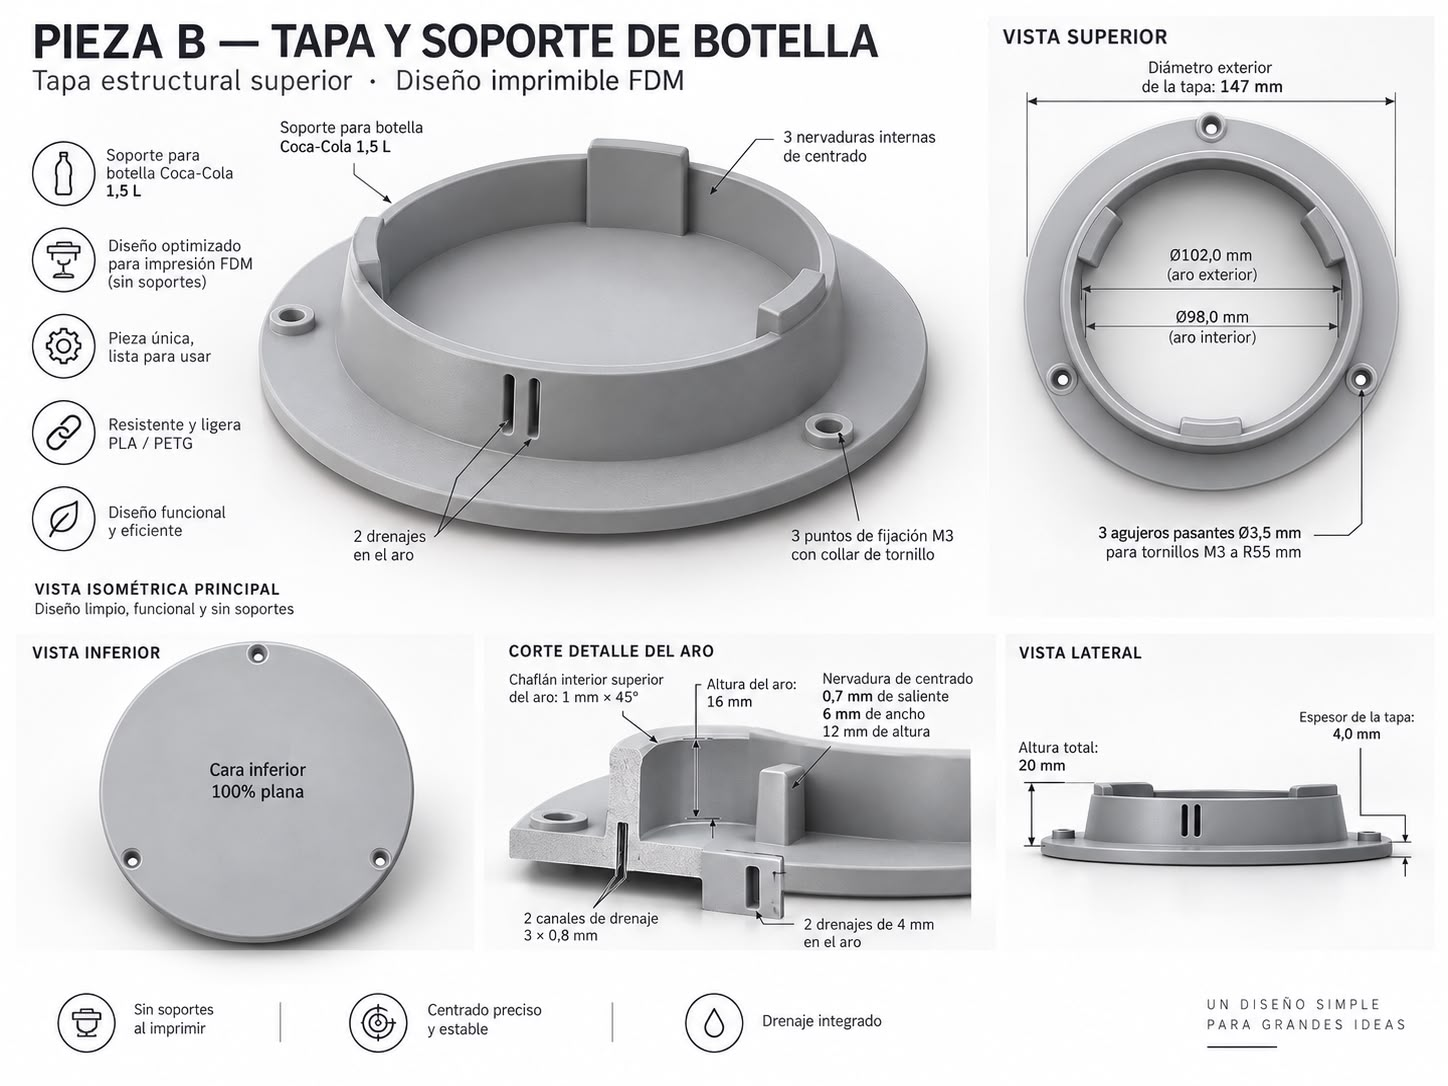
\includegraphics[width=\textwidth]{imagenes/botella_aireador.jpeg}
        \caption{Tanque PET con sensor sumergido y aireación.}
        \label{fig:tanque_pet}
    \end{subfigure}
    \hfill
    \begin{subfigure}[b]{0.48\textwidth}
        \centering
        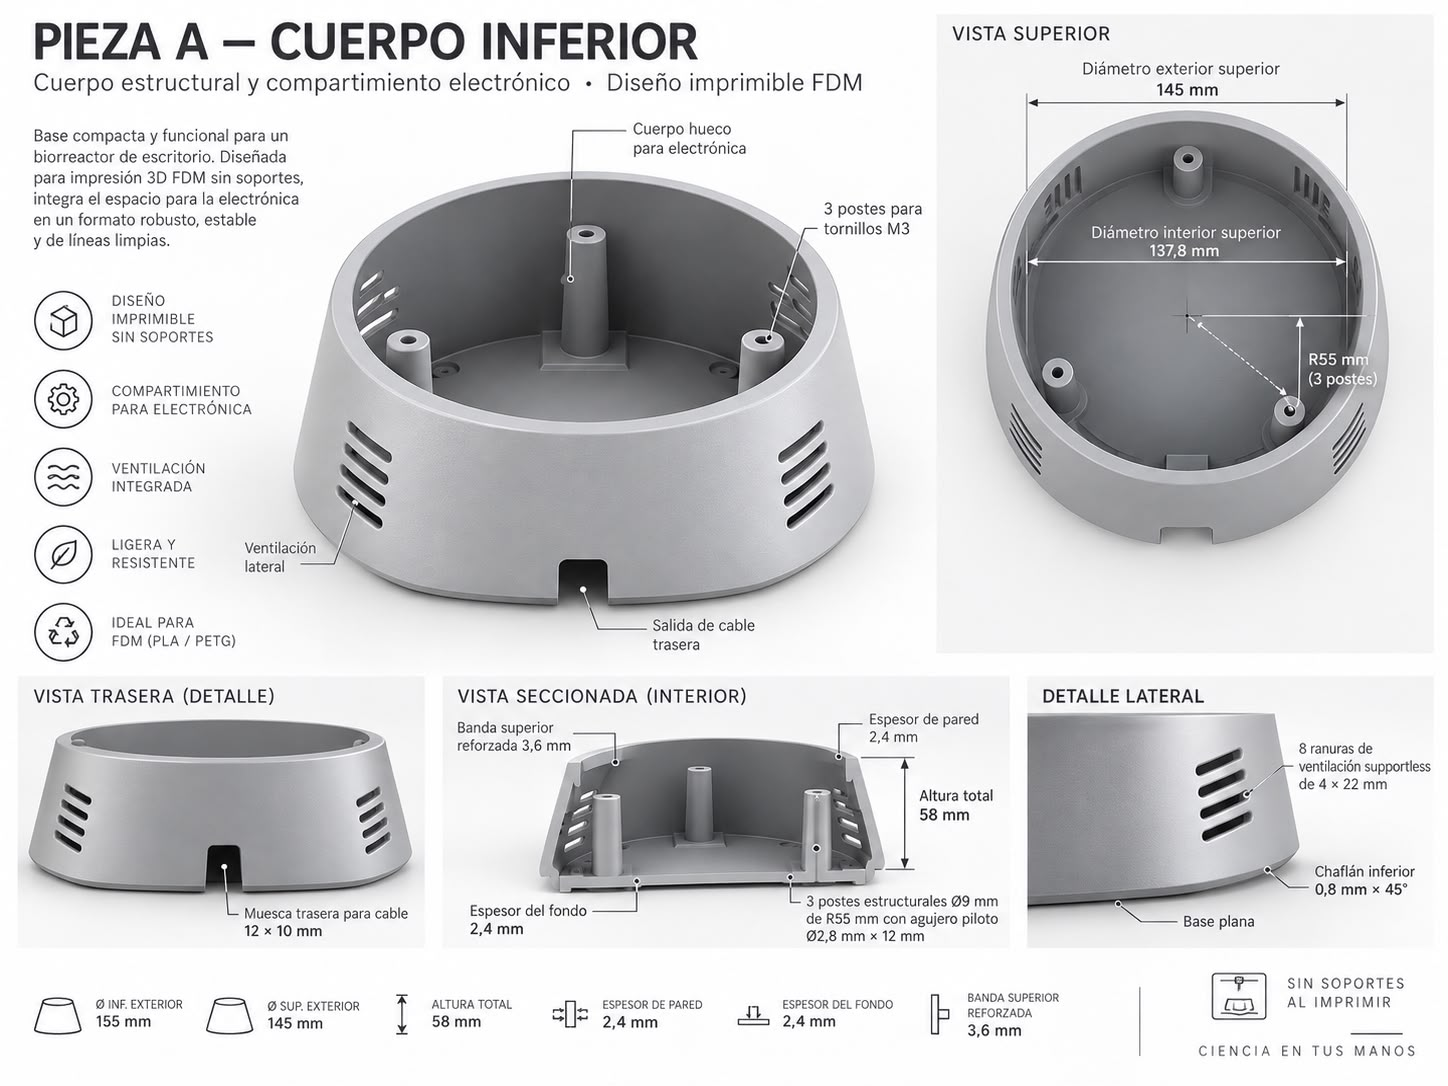
\includegraphics[width=\textwidth]{imagenes/acople_zuncho.jpeg}
        \caption{Acople mecánico de presión con zuncho metálico.}
        \label{fig:acople_zuncho}
    \end{subfigure}
    \\[0.3cm]
    \begin{subfigure}[b]{0.48\textwidth}
        \centering
        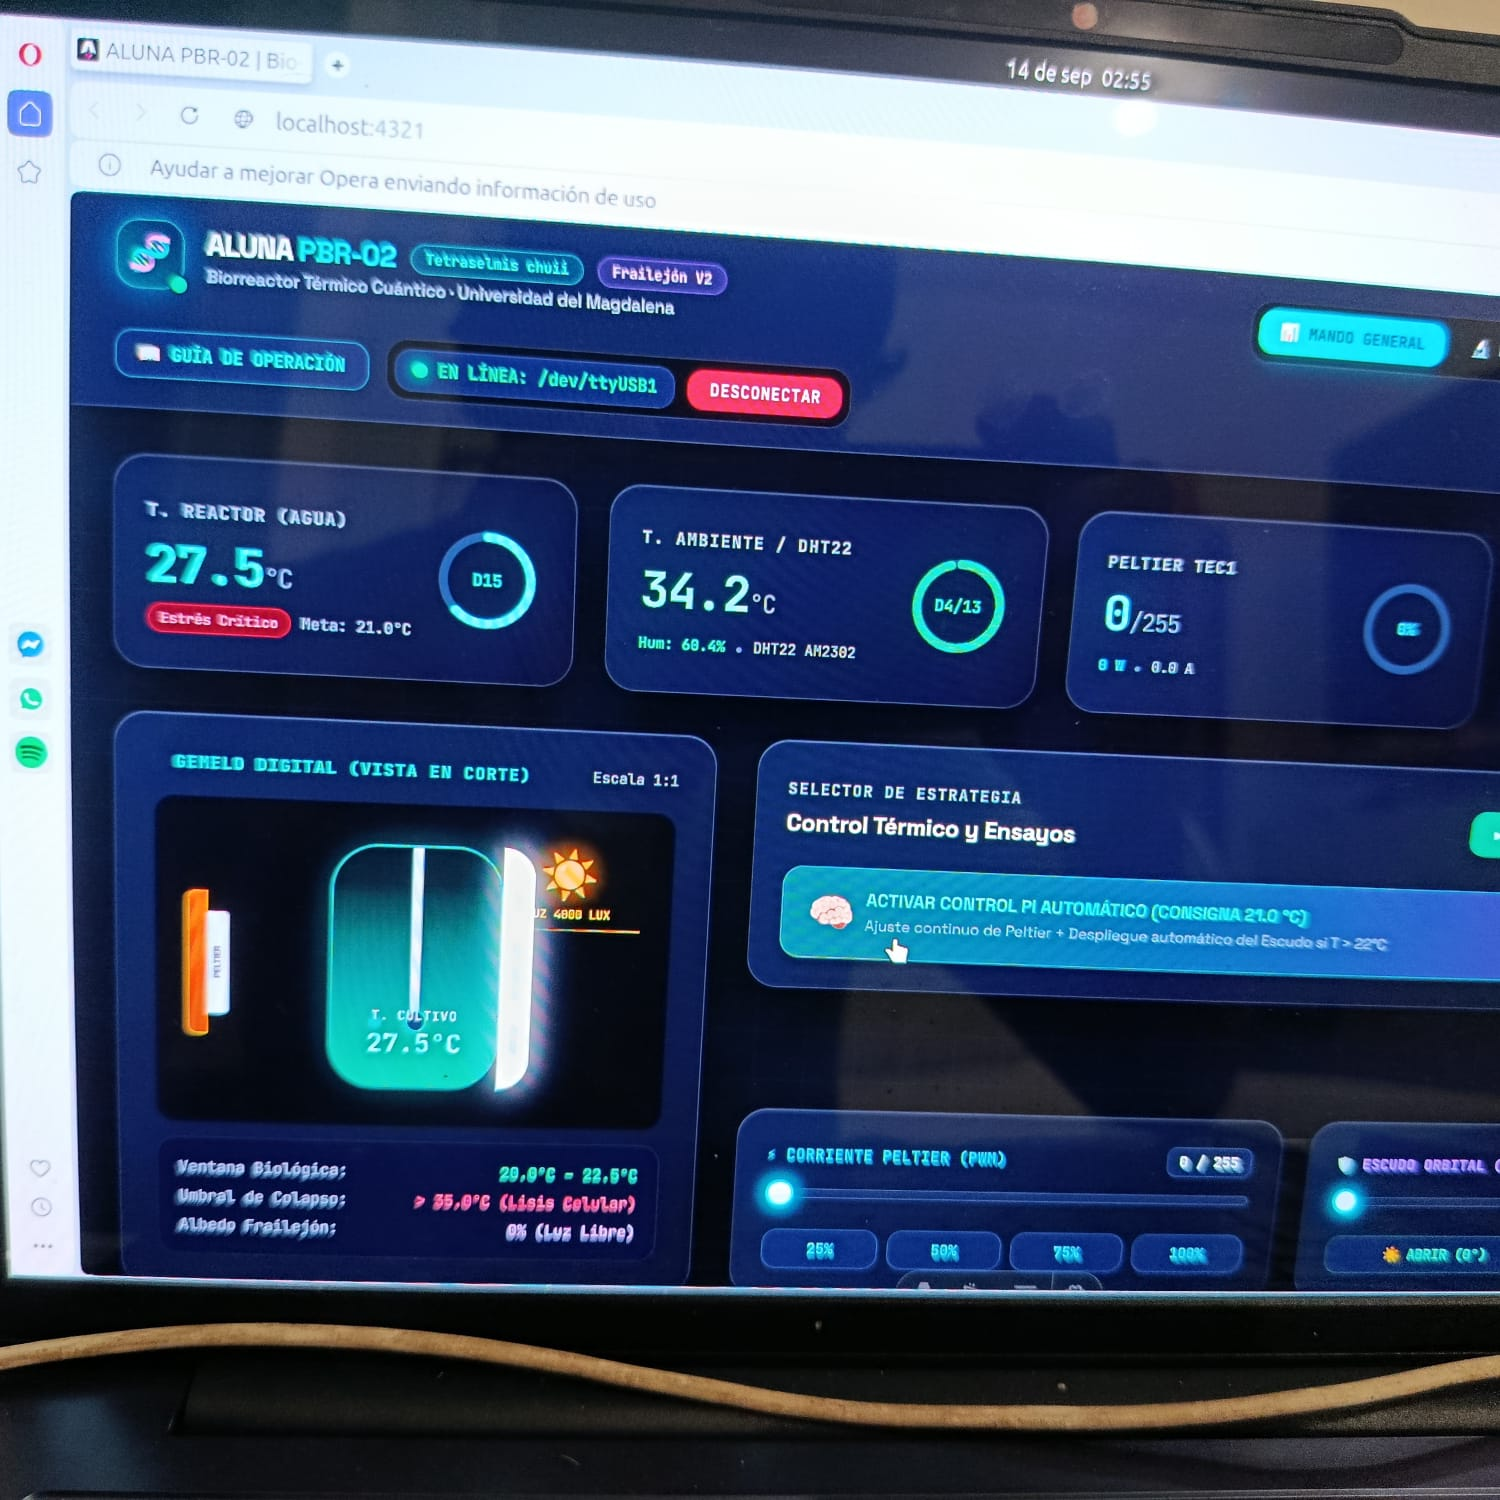
\includegraphics[width=\textwidth]{imagenes/disipador_kf200.jpeg}
        \caption{Disipador KF200-DGT con tubos de cobre.}
        \label{fig:disipador}
    \end{subfigure}
    \hfill
    \begin{subfigure}[b]{0.48\textwidth}
        \centering
        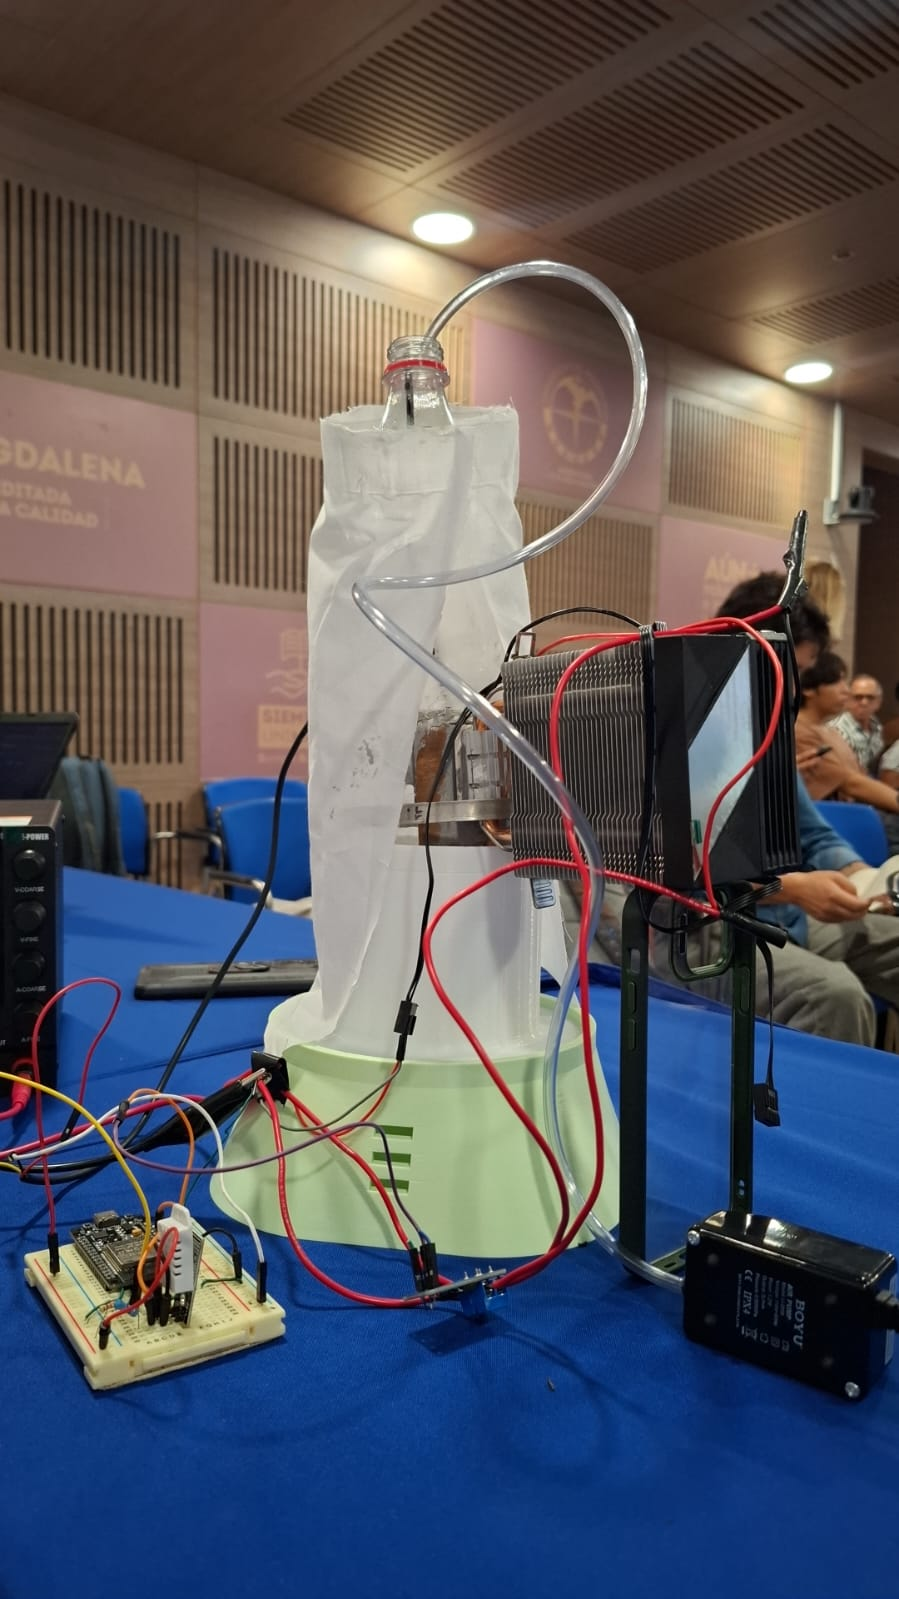
\includegraphics[width=\textwidth]{imagenes/prototipo_final.jpeg}
        \caption{Ensamble completo operando en banco.}
        \label{fig:prototipo_completo}
    \end{subfigure}
    \caption{Fotografías del proceso constructivo y ensamble final del fotobiorreactor ALUNA PBR-02.}
    \label{fig:galeria_fotos}
\end{figure}

\subsection{Registro Exhaustivo de Fallas Experimentales (Troubleshooting)}
Durante las pruebas de estrés en banco de trabajo, documenté, diagnostiqué y superé cuatro fallas críticas de ingeniería:

\subsubsection{Falla 1: Inversión de Polaridad en la Celda Termoeléctrica}
\begin{itemize}
    \item \textbf{Síntoma Observado:} Al energizar la etapa de potencia al 100\% PWM, los tubos de cobre del disipador descendieron bruscamente a temperaturas gélidas ($< 15\,^\circ\text{C}$), mientras que el agua del reactor comenzó a calentarse de forma acelerada ($> 30\,^\circ\text{C}$).
    \item \textbf{Diagnóstico Físico:} Por efecto Peltier, el sentido del flujo térmico depende exclusivamente de la dirección de la corriente continua. La polaridad en los bornes del módulo MOSFET estaba invertida, por lo que la celda bombeaba calor desde el ambiente hacia el reactor.
    \item \textbf{Solución Aplicada:} Inversión física de los terminales en las borneras \texttt{OUT+} y \texttt{OUT-} del MOSFET D4184, normalizando la extracción de calor desde el agua hacia el disipador exterior.
\end{itemize}

\subsubsection{Falla 2: Cuello de Botella Térmico por Conductividad del PET}
\begin{itemize}
    \item \textbf{Síntoma Observado:} La placa metálica de contacto alcanzaba temperaturas de escarcha ($< 2\,^\circ\text{C}$), pero la temperatura del agua descendía a una tasa muy lenta ($\approx 0.05\,^\circ\text{C/min}$).
    \item \textbf{Diagnóstico Físico:} El tereftalato de polietileno (PET) es un pésimo conductor térmico ($k_{\text{PET}} \approx 0.15 - 0.24\,\text{W/(m}\cdot\text{K)}$ frente a $k_{\text{Al}} \approx 205\,\text{W/(m}\cdot\text{K)}$ del aluminio). Además, las paredes expuestas de la botella absorbían continuamente calor por convección del ambiente cálido de Santa Marta ($32\,^\circ\text{C}$).
    \item \textbf{Solución y Ajuste:} Se aumentó la presión del zuncho para adelgazar la película plástica en el punto de contacto, se garantizó pasta térmica siliconada de alta densidad y se diseñó la adición de una camisa perimetral aislante de espuma elastomérica.
\end{itemize}

\subsubsection{Falla 3: Pérdida de Tensión y Limitación de Corriente por Resistencia de Contacto}
\begin{itemize}
    \item \textbf{Síntoma Observado:} Con la fuente fijada en $12.0\,\text{V}$, la celda Peltier consumía únicamente $1.8\,\text{A}$ en lugar de los $4.0\,\text{A}$ esperados según su hoja de datos.
    \item \textbf{Diagnóstico Eléctrico:} Concurrencia de dos fenómenos:
    \begin{enumerate}
        \item Los cables de prototipo (tipo Dupont) introducían una resistencia parásita no despreciable en serie ($R_{\text{cable}} \approx 0.5\,\Omega$).
        \item La tensión de compuerta $V_{GS} = 3.3\,\text{V}$ entregada por la ESP32 no saturaba completamente los canales de los transistores D4184 (que requieren $V_{GS} \ge 4.5\,\text{V}$ para $R_{DS(\text{on})}$ mínima).
        \item El Efecto Seebeck inverso genera una fuerza contraelectromotriz ($V_{\text{fem}} = \alpha_{te} \Delta T$) que se opone a la fuente a medida que la celda se enfría.
    \end{enumerate}
    \item \textbf{Solución Aplicada:} Sustitución del cableado de potencia por conductores de cobre de calibre AWG 18 soldados directamente, y ajuste de la tensión de la fuente de poder a $13.5\,\text{V}$, restaurando el consumo nominal en $3.8 - 4.1\,\text{A}$.
\end{itemize}

\subsubsection{Falla 4: Desincronización de Telemetría en el Dashboard Web}
\begin{itemize}
    \item \textbf{Síntoma Observado:} El servidor backend recibía tramas seriales válidas de la ESP32, pero las gráficas de ECharts en el navegador no se actualizaban y la consola arrojaba un error \texttt{ReferenceError: latest is not defined}.
    \item \textbf{Diagnóstico de Software:} La estructura de datos del endpoint REST fue refactorizada en el servidor para añadir campos, pero el frontend aún procesaba el formato anterior. Asimismo, desconexiones breves en el bus 1-Wire inyectaban valores nulos que interrumpían la gráfica.
    \item \textbf{Solución Aplicada:} Estandarización estricta del esquema JSON, corrección del mapeo en Astro y filtrado de lecturas espurias de bus abierto (como $-127.0\,^\circ\text{C}$ o $+85.0\,^\circ\text{C}$).
\end{itemize}

\newpage
\section{Conclusiones y Próximos Pasos Inmediatos}

\subsection{Conclusiones del Desarrollo Individual}
El desarrollo del fotobiorreactor automatizado ALUNA PBR-02 ha permitido demostrar que es factible diseñar, simular y construir un sistema de control de temperatura de grado científico para biotecnología marina con un presupuesto inferior a los \textbf{\$400.000 COP} (aproximadamente \$100 USD), frente a alternativas comerciales que superan los \$15'000.000 COP.

En el plano individual, los hitos consolidados bajo mi liderazgo técnico fueron:
\begin{enumerate}[itemsep=2pt, topsep=3pt, parsep=1pt]
    \item \textbf{Validación Teórica Integral en MATLAB/Simulink:} Se formuló e implementó exitosamente el modelo continuo de 4 EDOs no lineales (Droop + balance térmico Peltier). La generación procedural del modelo \texttt{aluna\_pbr\_simulink.slx} demostró que el mecanismo biomimético del Frailejón reduce el consumo eléctrico activo de la celda Peltier en más de un \textbf{40\%}.
    \item \textbf{Arquitectura Embebida de Alta Eficiencia:} El firmware programado en C++ para la ESP32 opera de forma totalmente asíncrona y no bloqueante, sincronizando dos sondas 1-Wire a 10 bits de resolución, un timer PWM por hardware a $1\,\text{kHz}$ y la cinemática de un servomotor MG996R sin pérdida de muestras ni retardos acumulativos.
    \item \textbf{Ecosistema IoT Operativo en Tiempo Real:} Se logró el despliegue exitoso del backend en Python (Flask) y el Dashboard web reactivo en Astro con visualizaciones de Apache ECharts, permitiendo supervisar el biorreactor, inspeccionar el gradiente térmico y operar actuadores de forma local y remota a 115200 baud.
    \item \textbf{Superación Experimental de Retos Físicos:} Se diagnosticaron y corrigieron exitosamente anomalías termodinámicas y eléctricas reales (inversión de polaridad Peltier, cuello de botella conductivo del PET y caídas de tensión por resistencia parásita), consolidando un banco de pruebas físicamente estable.
\end{enumerate}

\subsection{Próximos Pasos Inmediatos (Plan de Trabajo)}
Para culminar la transición del prototipo hacia su fase biológica activa, se ha establecido la siguiente hoja de ruta de ingeniería y validación experimental:

\begin{enumerate}[label=\textbf{Hito \arabic*:}, leftmargin=*, itemsep=2pt, topsep=3pt, parsep=1pt]
    \item \textbf{Finalización del Mecanismo de Apertura del Escudo Frailejón:}
    Culminar el acoplamiento cinemático entre el piñón metálico del servomotor MG996R y la pantalla semicilíndrica reflectiva de tela blanca ($0^\circ \to 180^\circ$) para automatizar el blindaje diurno frente a la sobre-irradiancia solar.
    
    \item \textbf{Mejora y Blindaje Térmico del Sistema Físico:}
    Instalar una camisa exterior de aislamiento térmico de espuma elastomérica sobre las caras de la botella PET que no están en contacto con la celda, y optimizar el puente térmico con pasta disipadora de alta conductividad ($>5.0\,\text{W/(m}\cdot\text{K)}$).
    
    \item \textbf{Caracterización FOPDT y Sintonía Definitiva Cohen-Coon:}
    Ejecutar una prueba ininterrumpida de respuesta al escalón en lazo abierto ($0 \to 100\%$ PWM) sobre el volumen real de agua para extraer experimentalmente los parámetros de ganancia $K$, constante de tiempo $\tau$ y retardo de transporte $L$, cargando los coeficientes sintonizados en el lazo digital de la ESP32.
    
    \item \textbf{Inoculación de la Cepa Viva (\textit{Tetraselmis chuii}):}
    Introducir el inóculo celular en medio estéril Guillard f/2 con aireación constante e iniciar la prueba biológica de 72 horas bajo fotoperiodo controlado (12h luz / 12h oscuridad) para evaluar la tasa de crecimiento celular y estabilidad osmótica a $21.0\,^\circ\text{C}$.
\end{enumerate}


\end{document}
